\documentclass[a4paper,11pt,twoside,openright]{report}

\usepackage{graphicx}
%\usepackage{ngerman}
\usepackage[utf8x]{inputenc}
\usepackage{fancyvrb}
\usepackage{courier}
\usepackage{helvet}
\usepackage{tikz}
\usepackage{xcolor}
\usepackage{pdfpages}
\usepackage[strict]{changepage}
\usepackage{indentfirst}
\usepackage{hyperref}

\pdfoptionpdfminorversion=6

% \definecolor{se_dark_blue}{RGB}{0,103,166} % powerpoint
\definecolor{se_dark_blue}{RGB}{0,96,178} % website
% \definecolor{se_light_blue}{RGB}{119,158,201} % powerpoint
\definecolor{se_light_blue}{RGB}{129,160,225} % website


%% setup listings
\usepackage{listings}
\lstset{
    numbers=left,
    numberstyle=\tiny,
    numbersep=5pt,
    xleftmargin=11pt,
    xrightmargin=4pt,
    frame=single,
    aboveskip=0pt,
    belowskip=-6pt,
    sensitive=true,
    float=!t,
    breaklines=false,
    captionpos=b,
    tabsize=2,
    showstringspaces=false,
    basicstyle=\small\ttfamily,
    morecomment=[l]{//},
    morecomment=[s][\itshape]{/**}{*/}
}

\setlength\parindent{24pt}

%% defines the listings laguage named 'MontiArc' derived from the language 'Java' 
%% adding the below listed keywords. See 
%% ftp://ftp.tex.ac.uk/tex-archive/macros/latex/contrib/listings/listings.pdf
%% for listings documentation
\lstdefinelanguage{MontiArc}[]{Java}{
  morekeywords={component, port, in, out, inv, package, import, connect, autoconnect}
}

% Seite einrichten
\setlength{\voffset}{-1in}
\setlength{\hoffset}{-1in}

\setlength{\topmargin}{2.5cm}		   
\setlength{\headheight}{0cm}		   
\setlength{\headsep}{0cm}		   
\setlength{\oddsidemargin}{3,3cm}  % innen ein wenig mehr Rand für die Klebebindung
\setlength{\evensidemargin}{2,7cm} % dafür außen ein wenig weniger
\setlength{\textwidth}{15cm}		   
\setlength{\textheight}{23,5cm}		   
\setlength{\parindent}{0cm}

\newcommand{\emptyLine}{{\LARGE ~\\}}

\begin{document}

% Einrücken von Absätzen verhindern und 1.5 Zeilen Absatzabstand
\setlength{\parindent}{0pt}
\setlength{\parskip}{1.5ex plus0.5ex minus0.5ex}

\renewcommand{\contentsname}{Table of contents}

%Dieses Teildokument beschreibt die Titelseite.
%

% Seitenzähler auf 1, Römische Ziffern.
\setcounter{page}{1}
\pagenumbering{roman}

\thispagestyle{headings}

%\changepage{<text height>}{<text width>}{<even-side margin>}{<odd-side margin>}{<column sep.>}{<topmargin>}{<headheight>}{<headsep>}{<footskip>}
\changepage{5,1cm}{2.4cm}{}{-0.7cm}{}{-2,3cm}{}{}{}

% Eigentliche Titelseite.
\begin{titlepage}
	
\begin{figure}\raggedleft
\includegraphics[height=3.0cm]{src/pic/logo.jpg}\end{figure}
  
\begin{tikzpicture}[overlay]

% horizontal lines
\draw[color=se_dark_blue, thick] (-1.6, 0.9) -- (17.4, 0.9);
\draw[color=se_light_blue, thick] (-1.4, 0.7) -- (17.4, 0.7);

% vertical lines
\draw[color=se_dark_blue, thick] (-1, 0.9) -- (-1, -24.5);
\draw[color=se_light_blue, thick] (-0.8, 0.7) -- (-0.8, -24.5);

\end{tikzpicture}

\vspace*{-1.5em}

\begin{flushleft}
  {\fontfamily{phv}  
  	{\LARGE
      RWTH Aachen University \\
      Software Engineering Group \\}
    \vspace{3em}
    
   {\LARGE \textbf{Workshop DSA}\\} 
   
   \vspace{3em}
   
   {\LARGE {Kölsch, Alexander}\\}
   \vspace{1em} 
   {\LARGE {Richter, Christoph}\\}
   \vspace{1em} 
   {\LARGE {Vasiljevic, Stefan}\\}
   \vspace{1em} 
   {\LARGE {Sommerhoff, Peter}\\}
   \vspace{1em} 
   {\LARGE {Strepkov, Ievgen}\\}
   \vspace{5em} 
   
   {\Large \textbf{Prüfer: Prof.\ Dr.\ B.\ Rumpe}\\}
   \vspace{1em} 
   {\Large \textbf{Betreuer: Klaus Müller, Andreas}\\}
   \vspace{7em} 

    {\large The present work was submitted to the Chair of Software Engineering \\}
    \vspace{1em}
    % The present work was submitted to the chair of software engineering
		{\large	Aachen, \today\\}
  }
  
  
  
\end{flushleft}

\end{titlepage}

\changepage{-5,1cm}{-2.4cm}{}{0.7cm}{}{2,3cm}{}{}{}





\graphicspath{{./src/pic/}}

\tableofcontents

% Ab erstem Kapitel Seiten arabisch zählen
\setcounter{page}{1}
\pagenumbering{arabic}

\clearpage

\chapter{Introduction}

In the context of the lecture \textit{Applied Software Engineering within the life cycle of Automotive Electronics} hold by \textit{Dr. Ansgar Schleicher} at \textit{RWTH Aachen University} we took part at a workshop organized by \textit{DSA - Daten- und Systemtechnik GmbH} \cite{DSA}.
The workshop was devided into two seperate topics: Extending the web \textit{portal BetoTrack} and the development of new functions for \textit{Vehicle Connectivity Gateway (VCG)} devices \cite{WorkshopDescription}. Within the VCG area we were allowed to choose between 3 different use cases: 
\begin{enumerate}
    \item Collision detection
    \item Theft detection
    \item Dead reckoning
\end{enumerate} 
At the workshop, we worked in the area of VCG development. We have decided to implement "Theft detection" use case because in our opinion it's the most interesting and useful case. In Germany, every 30 minutes had been stolen one car in 2014. 

Dead reckoning was a interesting topic we wanted to work on first. The downside was that many dead reckoning algorithms rely on sensors which are not available in the VCG (see section \ref{sec::vcg}). Dead reckoning often uses sensors like a compass and gyroscope to estimate the direction of movement \cite{kao1991integration}. Because of this we decided not to work at this topic.

The goal was to implement a C++ program which detects an attempted theft and reports it. We have used the preconfigured VirtualBox virtual machine with Eclipse IDE and the partially implemented project. We had to implement additional functional for the project, depending on the chosen use case.  The main device which we used to receive data for our program was VCG device. It provides functions like: 
\begin{enumerate}
	\item Location-Based functions : location and tracking of vehicles 
	\item Functions and status monitoring:  monitoring a status of vehicle, onboard diagnostic
	\item Update services : update some firmware
	\item Entertainment and communication services : access to the data in the cloud and communication services
	\item Safety functions : check of safety-relevant vehicle functions or crash-detection
	\item Predictive Maintenance : continuous recording of vehicle behaviour and sending data to central service for analysis and initiation of maintenance activity.
\end{enumerate}
For our purpose, we have used the acceleration sensor of the VCG, the GPS sensor, and information from FMS. We used WIFI network of VCG device to send compiled a program to VCG and receive information from it.\\
Our team consisted of 5 people and for higher efficiency, we decided to split the team into two sub-teams. First one worked on an algorithm of stealing detection and second team tried to get necessary data from the device. We applied pair-programming technic to achieve the better quality of the program.\\

\chapter{Used technology}

This chapter briefly describes the used technologies to implement a theft detection algorithm for vehicles. It introduces the Vehicle Connectivity Gateway and its web application Portal BetoTrack. After this the FMS standard is summarized.

\section{Vehicle Connectivity Gateway}
\label{sec::vcg}

The \textit{Vehicle Connectivity Gateway} (VCG) is a telematics and diagnostics unit. It connects a vehicle with different web portals and enables remote status monitoring of the vehicle as well as remote control actions. This unit can be build in cars, vehicles, trucks or agricultural machines \cite{VCG}.  

\begin{figure}[h]
    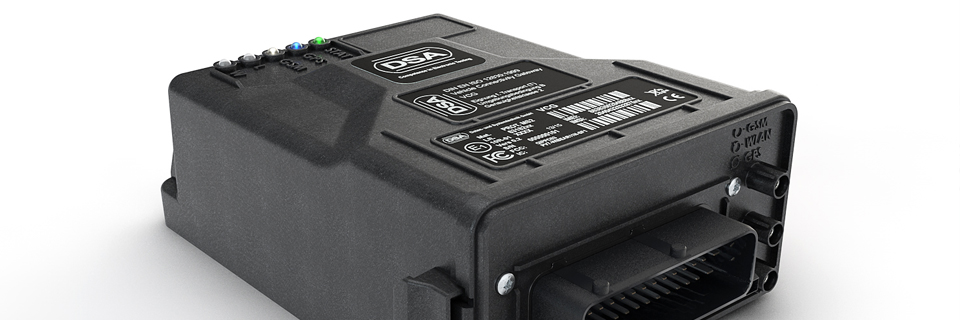
\includegraphics[width=1.0\textwidth]{src/pic/vcg_960x320px.jpg}
    \caption{VCG device \cite{DSA}}
\end{figure}

The VCG provides multiple communication mechanisms to transport data from the vehicle to the web:

\begin{itemize}
    \item GSM/UMTS Internet connection to the portal
    \item GPS/GLONASS satellite position detection
    \item WLAN for local diagnostics and additional functions
    \item One-Wire, RS232, digital and analog input for communication with sensors/transmitters
    \item CAN and Ethernet for ECU communication and diagnostics
\end{itemize}

Additionally the device has an build in accelerometer and build in battery to be independent of a vehicles power supply. We use the VCG to detect a theft of vehicles.

\section{Portal BetoTrack}
\label{sec::Portal}

Portal BetoTrack is a tracking web application which allows to track vehicles equipped with VCGs. The app can be displayed in a browser an shows different states of a vehicle \cite{BetoTrack}. 
In context of this workshop the theft detection results should be displayed in this portal. The implementation of this was done by other groups of the workshop.

\begin{figure}[h]
    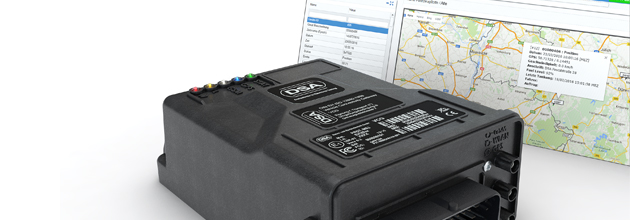
\includegraphics[width=1.0\textwidth]{src/pic/betotrack_630x220px.jpg}
    \caption{Portal BetoTrack \cite{BetoTrack}} 
\end{figure}

\section{Fleet Management System (FMS)}
\label{sec::FMSDef}

Fleet Management System (FMS) is a standardized interface for vehicle data. The FMS standard is supported by many big truck manufactures like Daimler, MAN Truck \& Bus, Scania, DAF Trucks, IVECO, Volvo Trucks and Renault Trucks \cite{FMS}.
The communication over the vehicle's CAN bus is standardized by the SAE J1939 network protocol.
FMS includes the following sensor values \cite{FMSStd}:

\begin{itemize}
    \item Vehicle improvement (all round)
    \item Vehicle speed (wheel based)
    \item Vehicle speed (from tachograph)
    \item Clutch switch (on/off)
    \item Brake switch (on/off)
    \item Cruise control (on/off)
    \item PTO (Status/Mode)
    \item Accelerator pedal position (0–100%)
    \item Total fuel used (litres since lifetime)
    \item Fuel level (0–100%)
    \item Engine speed
    \item Axle weight (kg)
    \item Total engine hours (h)
    \item FMS-Standard software version (supported modes)
    \item Vehicle identification number (ASCII)
    \item Tachograph information
    \item High-resolution vehicle distance
    \item Service distance
    \item Engine coolant temperature
\end{itemize}

Additional in version 2.0 the following values are also supported:
\begin{itemize}
    \item Environment temperature
    \item Driver ID
    \item Current fuel consumption
\end{itemize}

We use the FMS to have standardised values we can work with in our algorithm. In section \ref{sec::FMSUse} we describe which values we are using in our algorithm.


\clearpage

\chapter{Theft Detection}

\section{Use Cases}

We want to implement an algorithm which detects if a vehicle is stolen. Therefore we shortly explain the use cases we thought of. The user of the system wants to check if a theft alert is triggered via Portal (see section \ref{sec::Portal}). 
Figure \ref{fig::useCase} shows an overview of the use cases.

\begin{figure} [h]
    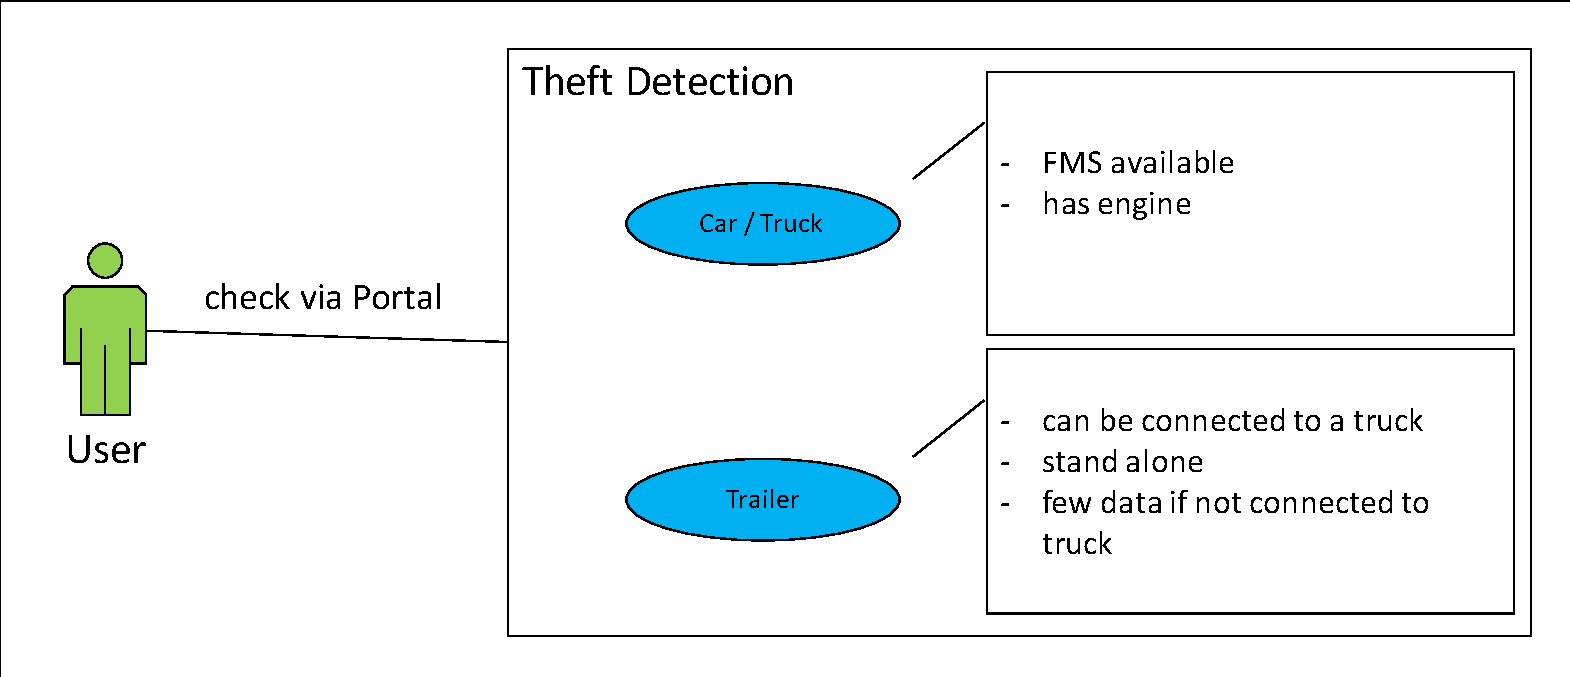
\includegraphics[clip, trim=0.1cm 0.1cm 0.1cm 0.1cm, width=1\textwidth]{src/pic/UseCase}
    \caption{Use Cases}
    \label{fig::useCase}
\end{figure}

We differentiate between theft detection for a) a car or truck, and b) a trailer only because VCGs are often built into trailers. Depending on these two cases, we have different data available which have to be considered in the implementation.

\clearpage

\section{Algorithm}
The algorithm works on a principle of the decision tree (see figure \ref{fig::decisionTree}) and it can be used for detecting a theft of either a car/truck or a trailer.


\begin{figure} [h]
    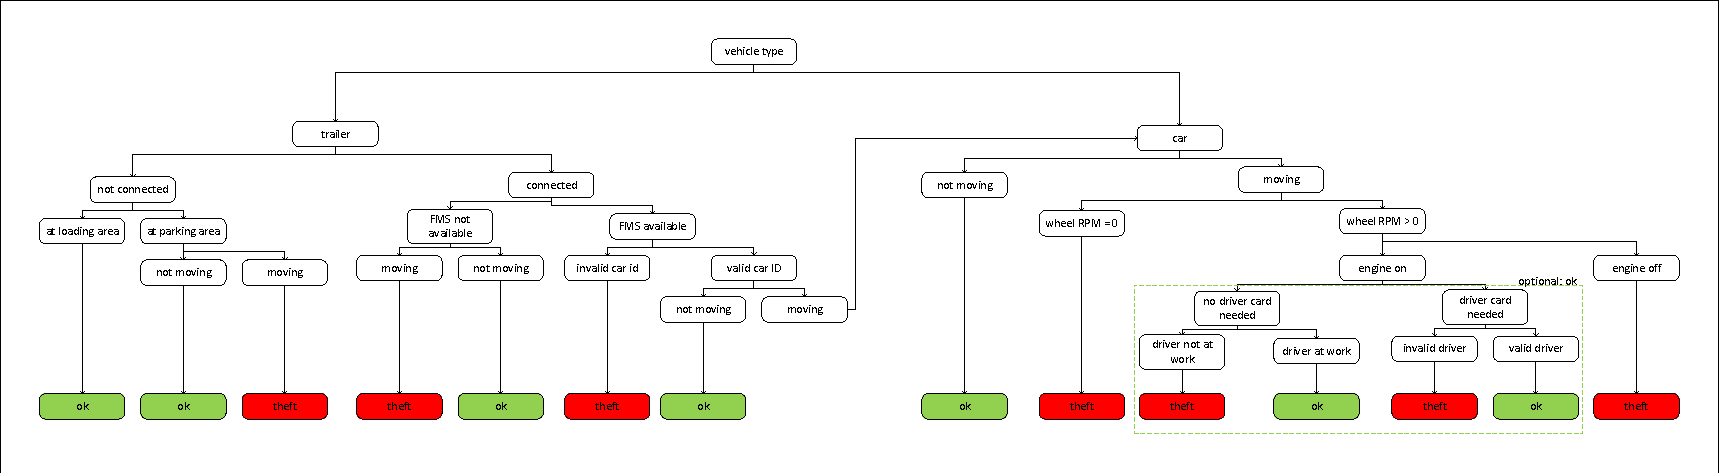
\includegraphics[clip, trim=0.1cm 0.1cm 0.1cm 0.1cm, width=1\textwidth]{src/pic/DecisionTree}
    \caption{Decision tree (the left and right sub-trees will be shown in more detail later)}
    \label{fig::decisionTree}
\end{figure}

Based on the whether a specific type of data is available (e.g. GPS location, driver card, wheel-based speed) and which state they are in (e.g. driver card is inserted or not), different paths in the tree are selected until a leaf is reached. The leaf is labeled with whether this configuration should be classified as a theft or not.

Since the use cases for trailer and truck are different, the algorithm will be explained for both cases independently (see Figure \ref{fig::decisionTreeTop}).

\begin{figure} [h]
    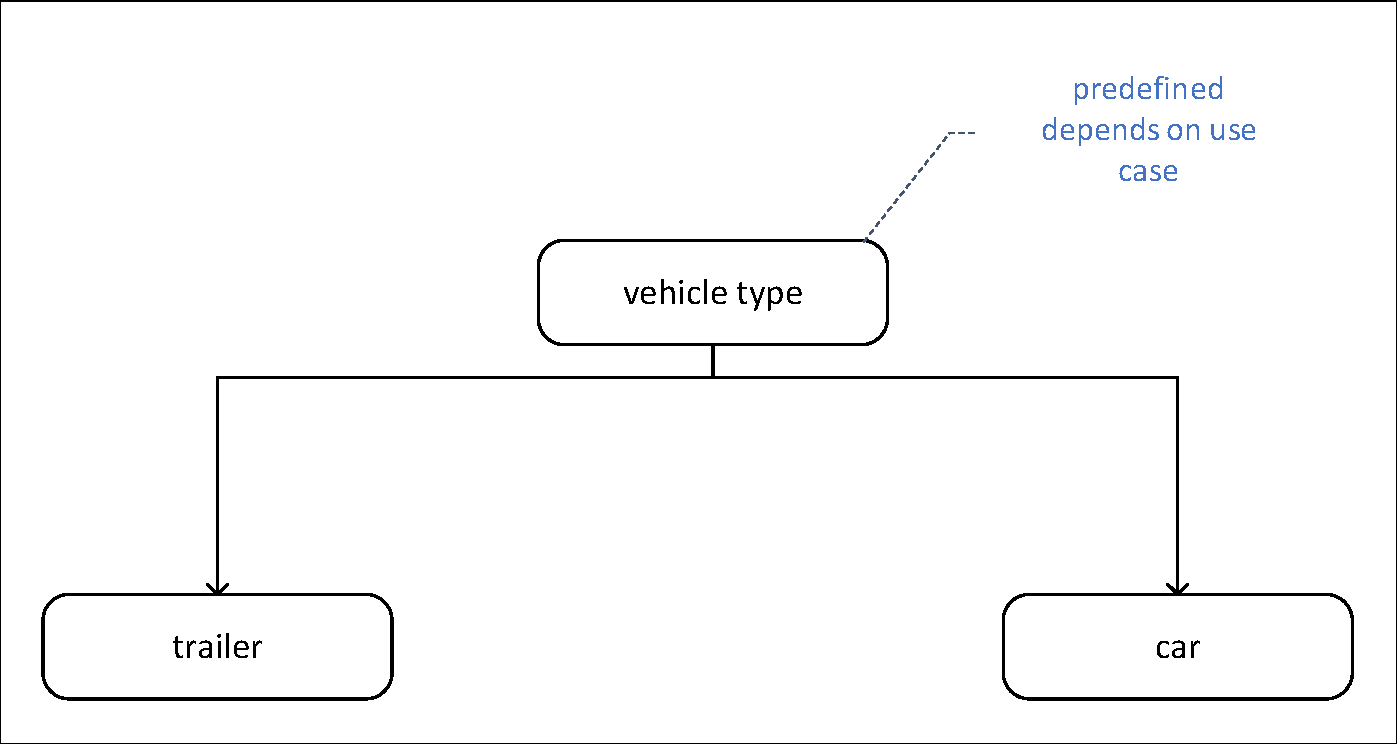
\includegraphics[clip, trim=0.1cm 0.1cm 0.1cm 0.1cm, width=1\textwidth]{src/pic/DecisionTreeTop}
    \caption{Decision tree top}
    \label{fig::decisionTreeTop}
\end{figure}

When the trailer case is considered, there exist specific properties that have to be taken into account in order to distinguish correctly between the possible outcomes. In other words, it has to be determined whether the trailer is connected to a vehicle, and whether FMS data is available, but also the current position of the trailer has to be acquired. 
The first decision is made according to the information of the power connection. If it is the external one, the trailer is not connected, which triggers a query on the current position. Under the assumption that the company that owns the trailer geofenced the loading and parking areas, further decisions are made. On the one side, while the trailer is located within the loading area, no potential theft is detected, regardless of whether the trailer is in motion or not. However, if the trailer is at a parking area, it is assumed that any kind of movement could represent the potential theft and the algorithm will end its path in the "theft detected" final node. The data needed for answering the previously described queries is acquired using the GPS and accelerometer sensors. The GPS is used for collecting the trailer location and checking whether the trailer is in the predefined position. It should be stated that our algorithm can easily be applied to the case when the trailer is being transported by a ship, where the geo-fence can be dynamically generated based on the boat position. When it comes to gathering the movement information, both the GPS and the accelerometer sensors are used. \\
In case that the trailer is connected to the vehicle, one additional resource is used for the algorithm analysis - the FMS data. If this data is not available and the trailer is moving, the theft is obviously detected, because the trailer is attached to an unrecognized vehicle. Again the movement information is acquired from the GPS/accelerometer sensors. However, if the FMS is available, that does not necessarily mean this is an acceptable case because a unique car ID is still to be checked. If it is an invalid id the stealing is detected, otherwise, the information of the vehicle movement is considered. At this point, the algorithm generates queries regarding the vehicle information only, therefore the theft of the car/truck analysis is to be described next and it follows below.

\begin{figure} [h]
    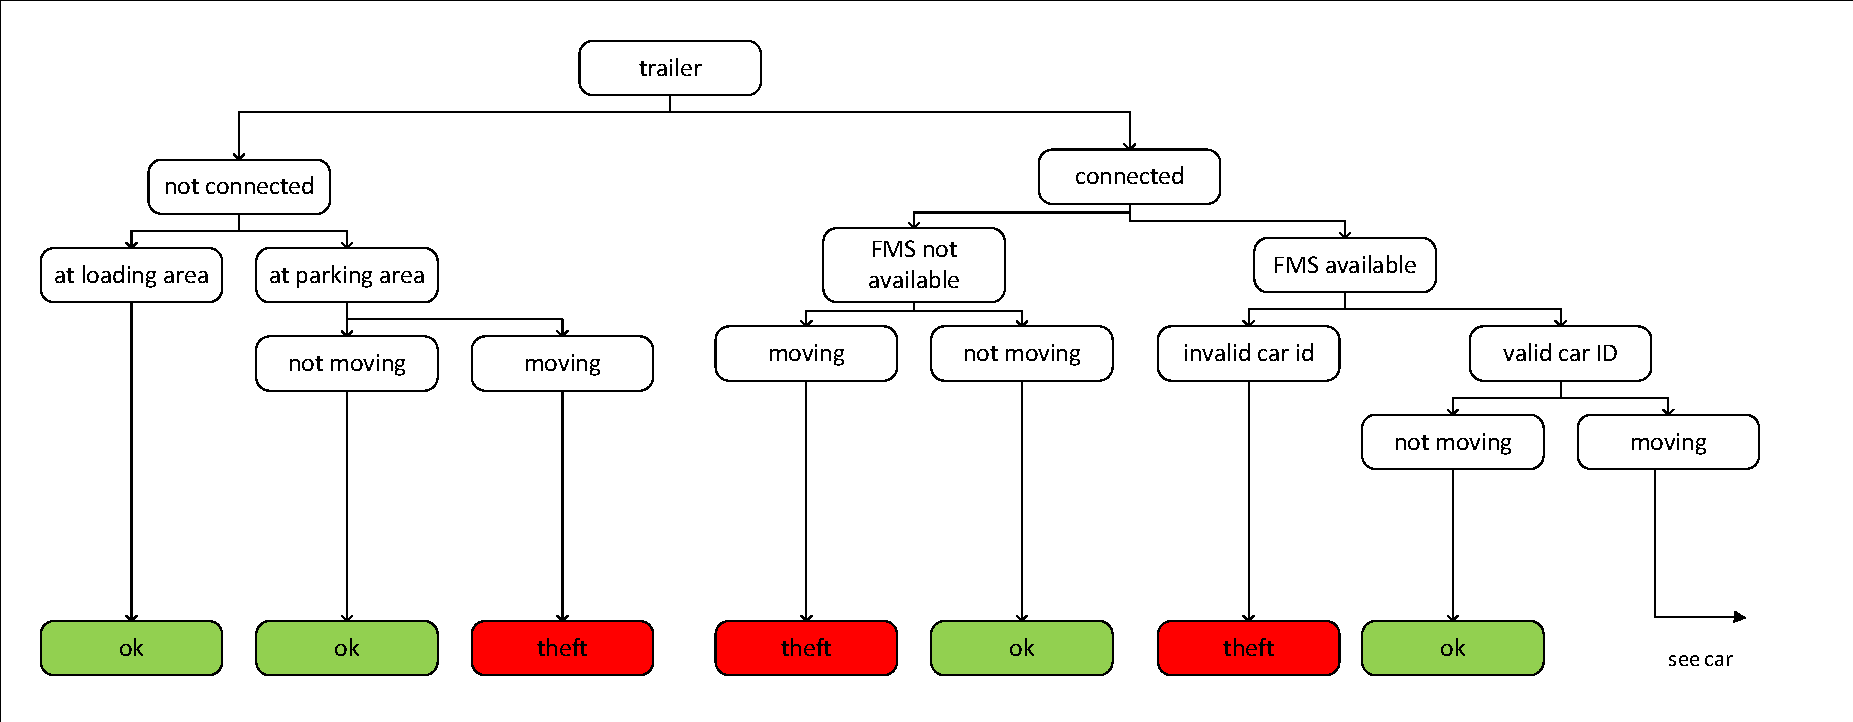
\includegraphics[clip, trim=0.1cm 0.1cm 0.1cm 0.1cm, width=1\textwidth]{src/pic/DecisionTreeTrailer}
    \caption{Decision tree trailer (left sub-tree)}
    \label{fig::decisionTreeTrailer}
\end{figure}

The GPS/accelerometer sensors answer the first important decision question in this part of the analysis - whether the car is moving or not. It is assumed that no motion represents a valid situation, so the only interesting case is recognizing the theft if there is a movement detected. Therefore, it is henceforth assumed that the vehicle is moving and the rest of the data that determines the path through the tree originates from the FMS. The wheel RPM is the first thing to check in this kind of situation because if the RPM is zero, the car is probably lifted and is being transported illegally. Otherwise, if the wheels are spinning, it should be asserted that the engine is on, which represents a valid scenario. Contrarily, if the engine is off with the RPM greater than zero, the theft is detected.\\
Moreover, if the driver cards are used in a company, the case when the engine is on can be extended in order to provide a more precise outcome. If a driver card is not required, it is checked whether the driver is on a job. If so, it is expected that the driver is in a vehicle, otherwise, the theft is identified. On the other hand, if the driver card is required, information on whether it is an invalid or a valid driver distinguishes between a theft and a regular situation. \\
In section 2.3 it will be explained thoroughly how the main data sources are used.

\begin{figure} [h]
    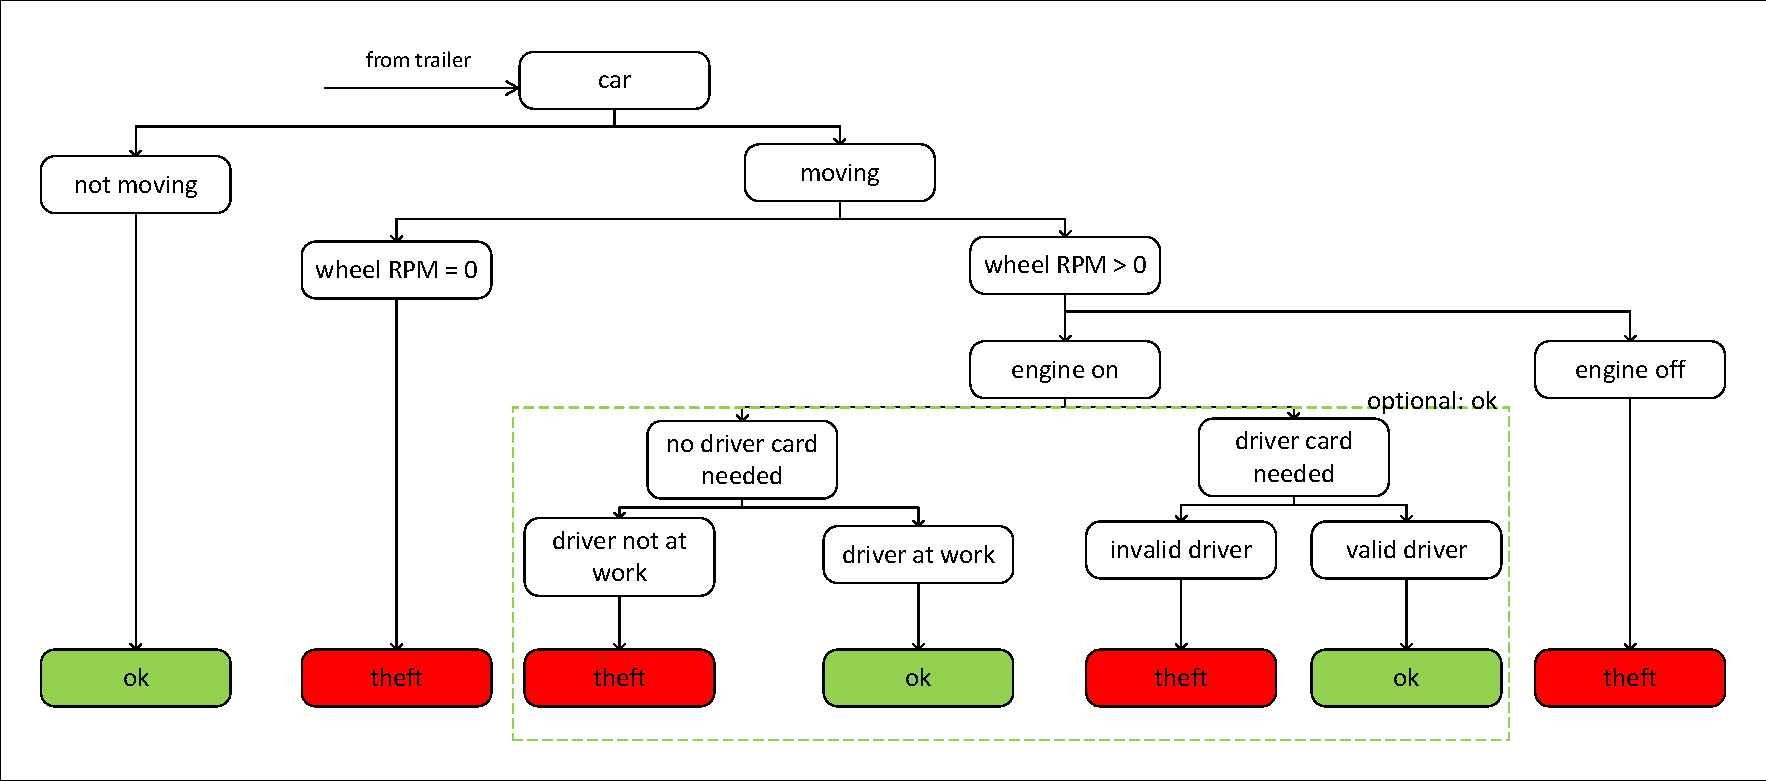
\includegraphics[clip, trim=0.1cm 0.1cm 0.1cm 0.1cm, width=1\textwidth]{src/pic/DecisionTreeCar}
    \caption{Decision tree car (right sub-tree)}
    \label{fig::decisionTreeCar}
\end{figure}



\section{Data Sources}

Based on our algorithm idea represented by the decision tree, we knew which data we needed to implement our theft detection algorithm. In this chapter, we discuss in more detail how we extracted the data from the vehicle and encapsulated it in our code.

\subsection{Accelerometer}
The first data source we used was the vehicle accelerometer which emits the current acceleration in X, Y and Z direction every 100ms by default. We chose to extract this data first because it can be used to implement a simple but effective theft detection already. Every illegal movement of the device (and thus vehicle) will be reflected in the accelerometer data.

In order to get access to the accelerometer data, we used a C++ library dedicated to the BMA255 accelerometer \cite{BMA255} built into the test devices. The basic procedure to read data from it is as follows:

\begin{enumerate}
	\item Open connection via \texttt{open("/dev/bma255", O\_RDWR)}
	\item Use the \texttt{select()} and \texttt{FD\_ISSET()} functions to check if data can be read from the file descriptor
	\item Read the available data via \texttt{int numberRead = read(accelerationHandle, buffer, length - 1);} with a buffer of the right size
\end{enumerate}

We can parse the resulting data to retrieve the X, Y and Z acceleration. Naturally, reading has to occur continuously to read the current values. We decided to encapsulate the basic data access as above into a class \texttt{AccelerometerSensor} and add another proxy layer on top which persists the 5 most recent data points and calculates whether the vehicle is moving based on these. We adjusted the threshold until we were satisfied with the behavior but future work remains in this area.

\subsection{GPS}
In order to implement further layers of theft protection, we need to incorporate GPS data. This way, we can detect a theft if the vehicle is moving but the wheels are not spinning for example. To extract GPS data from the device, we used the GPSd daemon \cite{GPSd} for C/C++. The procedure to access the data uses file descriptors again and is thus similar to the accelerometer.

GPSd provided various values of which we only need a small subset. Thus, we encapsulated the values we need into a \texttt{gps\_data} struct to constrain the thousands of values provided by FMS to those we need and increase performance. Also, we again added another proxy layer which calculates the distance between two data points from GPS and decides whether the vehicle is moving.

\subsection{FMS}
\label{sec::FMSUse}
For commercial vehicles, additional data from the Fleet Management System (FMS) is available (see section \ref{sec::FMSDef}). This can be used e.g. to check whether a valid driver card has been inserted (indicating that the designated driver is present) or not (indicating that the vehicle is moving without its driver). All relevant data for our algorithm are:

\begin{itemize}
	\item \textbf{The FMS status} to check whether FMS is currently not connected or online
	\item \textbf{The battery ECU power state} to check if a trailer is connected to its truck or not
	\item \textbf{The vehicle ID} to verify with a whitelist
	\item \textbf{The engine speed} to see whether the engine is running or not
	\item \textbf{The wheel-based speed} to decide whether the wheels are spinning or not
	\item \textbf{The driver card state} to check whether a valid driver card is present or not
	\item \textbf{The driver status} to check whether the driver is currently not at work, working, on a break, etc.
\end{itemize}

Again, we encapsulated these values we need into a struct called \texttt{fms\_data} to constrain the thousands of values provided by FMS to those we need. This also acts as documentation for which values are used and transmitted across the classes. For FMS, we do not need a proxy class because we only need the actual values coming directly from FMS.

\vspace{.5cm}

For all data access, we made sure to open the connection only once, then continuously read data, and then close the connection in the destructors of the appropriate classes. Also, we refactored our architecture to use singletons for the accelerometer and GPS sensor classes because we really only need one instance of both and this can prevent accidental use of copy constructors.



%\includegraphics[width=0.8\linewidth]{3.jpg}
\section{Architecture}

As described before, the three main data sources that the algorithm uses are FMS bus, accelerometer sensor and GPS sensor. Since the overall available data is much larger than the data required by the algorithm, the corresponding API is provided for each data source. In addition to the encapsulation role these interfaces have, they can be extended for the future use as well, in the case of additional modifications or improvements. Moreover, a layer is added above the accelerometer and GPS API in order to maintain the acquired data and provide further actions.
\begin{figure}[!htb]
	\makebox[\textwidth]{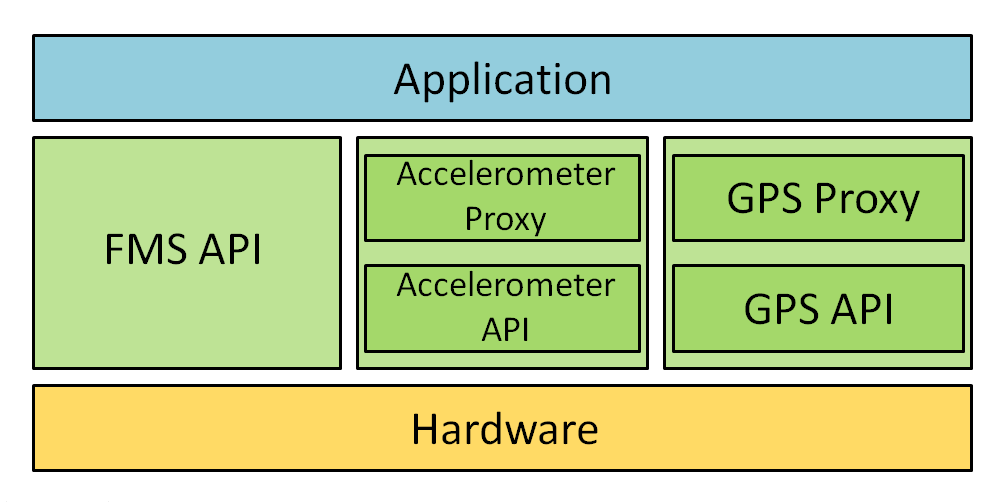
\includegraphics[width=\textwidth]{architecture}}\caption{Architecture}
    \label{fig::architecture}
\end{figure}
\\
As it is shown in the Figure \ref{fig::architecture}, the architecture is layer based. The higher layers abstract from lower layers, while the lower layers do not know about higher layers. Nevertheless, not all the communication links are permitted. Allowed ones are only the module based communication links into the directly lower level. That being said, neither the horizontal communication nor bypassing the layers is permitted. Currently, the only present communication is top-down by function calls, but the possible one could also be bottom-up by triggering some event. This structure improves the maintainability and scalability on the one hand, but in contrast, it could increase a communication load significantly with including more functions to the algorithm. 
\clearpage


\chapter{Evaluation}

% What are the results?
% Whats works good?
At the end of the workshop, we were able to have our algorithm idea implemented. Due to the timeframe of the workshop, we were only able to manually test the essential functions, i.e. theft detection via the accelerometer and suspicious GPS movements. As soon as the device is moved (e.g. lifted up from a table), the accelerometer-based detection correctly fired. Additionally, we field-tested the GPS-based detection by running down the street to simulate a noticeable change in location.

However, in the scope of the workshop, much of the FMS data was not available. Thus, not all branches from our decision tree could be tested. This could have been achieved by simulating the FMS data. However, we did not have the necessary time left towards the end of the workshop.

% Where are weaknesses in the algorithm? (Stolen vehicle with key)
Theft detection is a challenging problem. Even though all the different branches in our decision cover many possible ways to steal a vehicle, there are cases which are not covered -- and cases that are hard to detect in general. This includes the case where a thief has gained access to the vehicle keys, thus leaving no way to detect a theft in non-commercial vehicles (which do not require a driver card).


\clearpage

\chapter{Conclusion and Future Work}
Our concept and the implementation on the VCG show, that a theft detection for a vehicle or a trailer - equipped with a VCG - is realizable and that even basic concepts can be used for this safety-critical use case. With the help of our tests we can say, that our approach is working under testing conditions. But in our program, only basic functions for theft detection are implemented, which are necessary for the correct operation of the program. Still, some weak points remain which can be improved in the future. These points are:

\begin{itemize}
	\item Use binary mode to read from acceleration sensor to avoid parsing the data manually as a string
	\item Calibrate acceleration sensor threshold based on in-the-field testing (e.g. beside a highway)
	\item Test all branches of the algorithm, ideally with real vehicle data
\end{itemize}

The problem with parsing the data is, that the algorithm could not react on wrong input data or detect an knock event at the moment. A knock event is send by the box, if someone knocks on it. Wrong input data could occur, if the connection to the sensor is disturbed or the sensor is damaged. In these cases, the algorithm throws an exception, because it can not handle the data. The binary mode can solve these problems. Anther weak point is the threshold of the acceleration sensor. The threshold is generated from data, which was measured while the box was lying on a table, so that there weren't any disturbing factors. In a real environment are many vibrations and disturbing signals, so that the threshold will be to low. But the exact threshold has to be measured during an field test. A test inside a trailer on a rest area near a highway will be quite useful, because other trucks will pass the test arrangement with a high speed and will generate lots of vibrations. The last problem, which occurs during the workshop, was, that the FMS system was not working correctly. It had only dummy data for some values. These tests have to be repeated under real conditions with a working FMS system and real vehicle data to make sure, that everything of the algorithm works correctly.

In addition to that issues, there are two concrete ideas for an improved theft detection algorithm. The first approach is an extended geofencing. In our concept, the geofencing is only used for the detection, if a trailer is inside a loading area, for example a train station or a harbor. But there are different use cases, where the trailer is moving and it is not a theft. Examples are a trailer loaded on a train or a ship. Therefore, the geofencing can be extended on railroad lines or ship routes. Another idea is to deactivate the theft detection during the transport. The second improvement for our algorithm is the usage of information from the portal. The portal delivers information about the working time of the drivers. Combined with the truck, an improved algorithm could check, if the truck or truck/trailer combination is moving, although the responsible driver for the truck is currently not working. 

These two issues and the two ideas show, that there are several improvements for our concept, which can be designed and implemented in future work.

\clearpage

\end{document}
